% ============================================================================================
% BAB III ANALISIS MASALAH
% ============================================================================================
\cleardoublepage
\chapter{ANALISIS MASALAH}
\label{chap:analisis-masalah}

Bab ini menyajikan analisis terhadap sistem inspeksi kontainer yang ada saat
ini, identifikasi kebutuhan sistem, eksplorasi alternatif solusi konseptual, dan
justifikasi pemilihan solusi berdasarkan kriteria objektif. Analisis ini menjadi
fondasi untuk perancangan arsitektur konseptual yang dipaparkan pada Bab IV.

\section{Analisis Sistem Saat Ini}

Analisis sistem saat ini dilakukan untuk mengidentifikasi keterbatasan mendasar yang menjadi akar permasalahan arsitektural, sehingga kebutuhan sistem yang dirumuskan kemudian merespons celah yang teridentifikasi.

\subsection{Model Konseptual Sistem Inspeksi Kontainer Saat Ini}

Sistem inspeksi kontainer yang berlaku saat ini dapat dianalisis melalui kerangka \textit{People–Process–Technology–Data} untuk memahami komponen utama dan interaksinya. Kerangka ini memungkinkan identifikasi sistematis terhadap keterbatasan pada setiap dimensi, sehingga rancangan solusi dapat merespons seluruh aspek masalah secara holistik.

\textbf{Dimensi manusia.}
Dimensi manusia melibatkan beberapa aktor dengan kepentingan dan tanggung jawab
yang berbeda:

\begin{enumerate}
  \item Petugas inspeksi pelabuhan melakukan pemeriksaan fisik kontainer
  berdasarkan \textit{checklist} manual dan pengalaman personal.
  \item Petugas Bea dan Cukai berperan dalam verifikasi kepatuhan terhadap
  regulasi kepabeanan dan keamanan.
  \item Supervisor operasional mengawasi proses inspeksi serta mengelola
  alokasi sumber daya.
  \item Operator terminal mengelola alur kontainer di area pelabuhan dan
  berinteraksi dengan \textit{Terminal Operating System}.
  \item Pemilik barang membutuhkan informasi status inspeksi untuk mendukung
  koordinasi logistik.
\end{enumerate}

Ketergantungan penuh pada interpretasi manual menyebabkan variasi hasil
inspeksi antarpersonel, terutama ketika kategori kerusakan, tingkat keparahan,
dan dasar keputusan tidak dicatat dalam struktur data yang sama. Tidak adanya
mekanisme standardisasi atau panduan objektif terintegrasi memperkuat sifat
subjektif dari proses penilaian kerusakan.

\textbf{Dimensi proses.}
Dimensi proses menggambarkan alur inspeksi yang masih mengikuti pola
sekuensial sebagai berikut:
\begin{enumerate}
  \item Kontainer masuk ke area pelabuhan dan dicatat dalam sistem administrasi
  terminal.
  \item Petugas melakukan pemeriksaan visual berdasarkan \textit{checklist}
  keamanan seperti CTPAT 7-Point Container Inspection Checklist atau panduan
  kondisi kontainer seperti IICL.
  \item Hasil pemeriksaan dicatat melalui dokumen kertas, formulir lapangan,
  atau pencatatan mobile yang berdiri terpisah dari sistem inspeksi terpadu.
  \item Supervisor meninjau hasil inspeksi sebelum kontainer diizinkan keluar
  dari area pelabuhan.
  \item Data inspeksi dimasukkan ulang ke sistem TOS atau dikirim melalui surat
  elektronik kepada pemangku kepentingan.
\end{enumerate}

Ketiadaan standar formal untuk penilaian kerusakan maupun dokumentasi terstruktur yang terintegrasi dengan alur informasi pelabuhan mengakibatkan fragmentasi proses dan inkonsistensi keluaran. Setiap tahapan dilakukan secara manual tanpa dukungan sistem yang memvalidasi kelengkapan atau kebenaran data.

\textbf{Dimensi teknologi.}
Dimensi teknologi mencerminkan keterbatasan sarana pendukung sistem saat ini:

\begin{enumerate}
  \item \textit{Checklist} kertas atau formulir daring/internal sederhana belum memiliki
  validasi otomatis maupun panduan standar yang terintegrasi.
  \item \textit{Terminal Operating System} mengelola pergerakan kontainer di
  dalam terminal, tetapi belum menerima data inspeksi secara otomatis.
  \item Pertukaran informasi masih mengandalkan kanal komunikasi dan berkas
  operasional terpisah tanpa mekanisme pelacakan formal.
\end{enumerate}

Tidak ada komponen yang memfasilitasi standardisasi proses, pencatatan
terstruktur, atau integrasi lintas sistem. Akibatnya, informasi inspeksi
tersebar dalam format heterogen dan memerlukan konsolidasi ulang manual sebelum
dianalisis. Jenis platform
pencatatan mobile tidak diidentifikasi sebagai aplikasi tertentu karena bukti
observasi tidak menunjukkan identitas platform secara jelas dan akses ke sistem
internal dibatasi oleh kerahasiaan operasional.

\textbf{Dimensi data.}
Dimensi data menunjukkan keterbatasan kualitas dan riwayat informasi
inspeksi:

\begin{enumerate}
  \item Data dicatat dalam format bebas tanpa skema standar.
  \item Data tidak disertai mekanisme \textit{audit trail} yang mencatat siapa
  melakukan inspeksi, kapan inspeksi dilakukan, dan kriteria apa yang digunakan.
  \item Data inspeksi masih terisolasi dari sistem TOS, PCS, atau Inaportnet.
  \item Interpretasi hasil inspeksi bergantung pada subjektivitas petugas
  individual dan tidak memiliki dasar metadata yang memadai untuk dipertahankan
  sebagai informasi yang konsisten.
\end{enumerate}

Ketiadaan \textit{metadata} dan mekanisme riwayat kontainer membuat data
inspeksi tidak dapat langsung dimanfaatkan untuk analisis tren ataupun audit
kepatuhan.

\subsubsection{Bukti Observasi Lapangan}

Analisis kondisi eksisting didukung oleh dokumentasi lapangan yang menunjukkan
empat pola utama: inspeksi fisik pada kontainer, penggunaan dokumen cetak,
pencatatan melalui perangkat mobile, dan interaksi manual pada titik layanan
operasional. Bukti visual tersebut digunakan untuk menyimpulkan karakter proses,
bukan untuk membuka isi data operasional yang bersifat terbatas. Oleh karena
itu, isi dokumen, identitas kontainer, dan detail formulir internal tidak
ditampilkan secara penuh pada naskah ini.

\begin{figure}[ht]
  \centering
  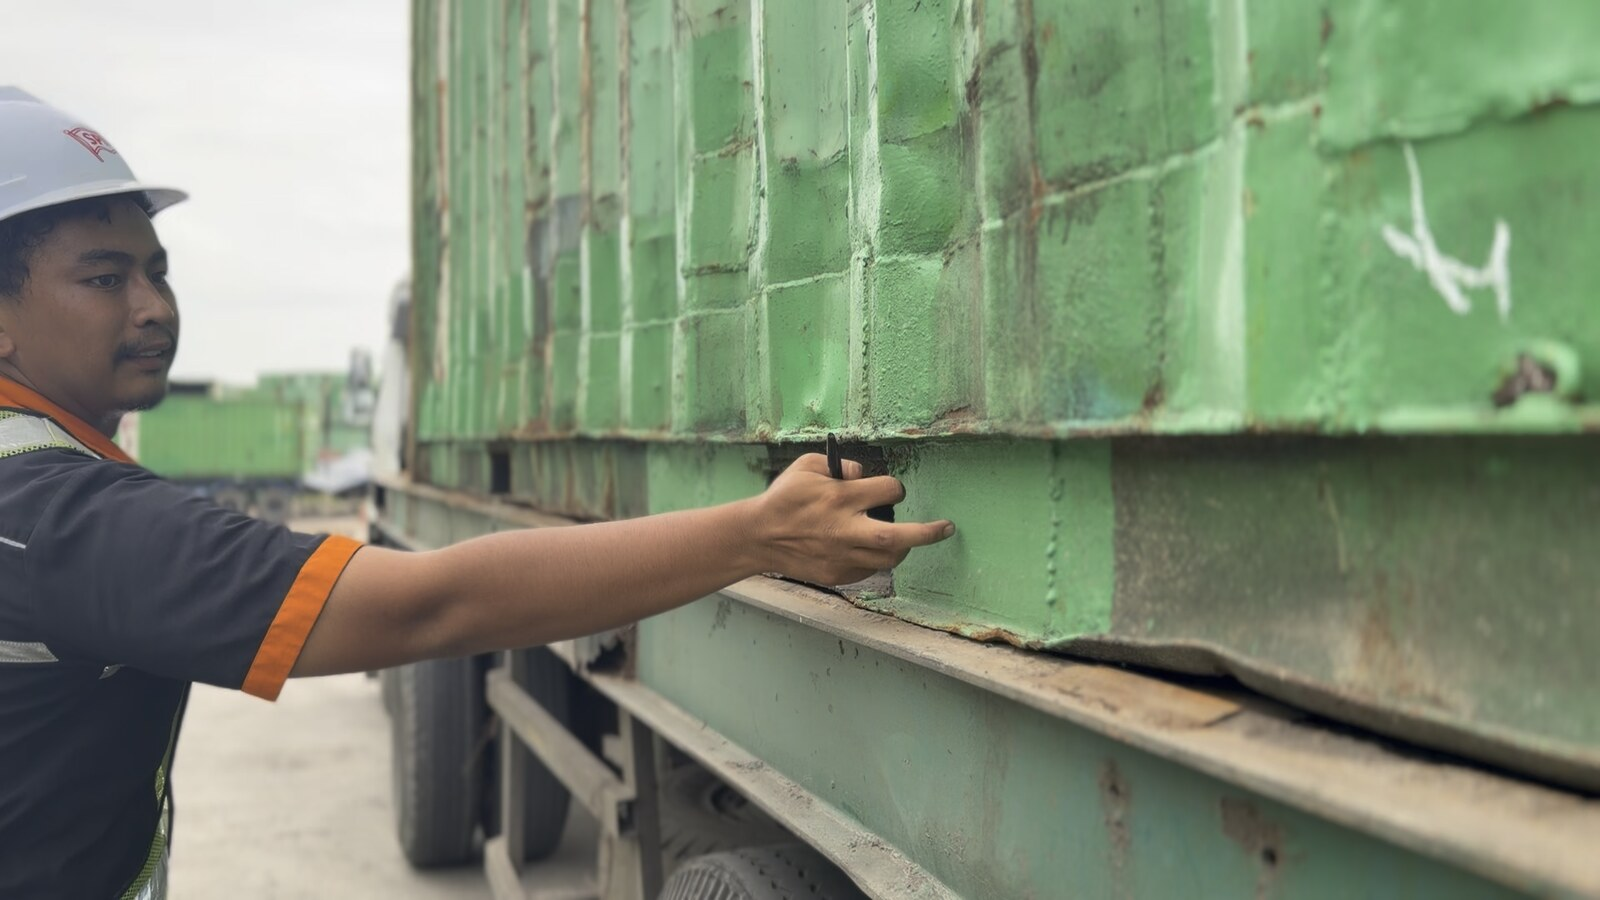
\includegraphics[width=0.9\textwidth]{images/evidence-eksisting-inspeksi-fisik.jpg}
  \caption{Dokumentasi observasi pemeriksaan fisik pada sisi kontainer}
  \label{fig:evidence_eksisting_inspeksi_fisik}
\end{figure}

Gambar~\ref{fig:evidence_eksisting_inspeksi_fisik} menunjukkan bahwa proses
inspeksi masih melibatkan pemeriksaan visual langsung pada permukaan kontainer.
Kondisi ini memperkuat kebutuhan rancangan terhadap akuisisi bukti visual,
standardisasi kriteria pemeriksaan, dan pengaitan hasil inspeksi ke identitas
kontainer yang sama.

\begin{figure}[ht]
  \centering
  \begin{subfigure}[t]{0.32\textwidth}
    \centering
    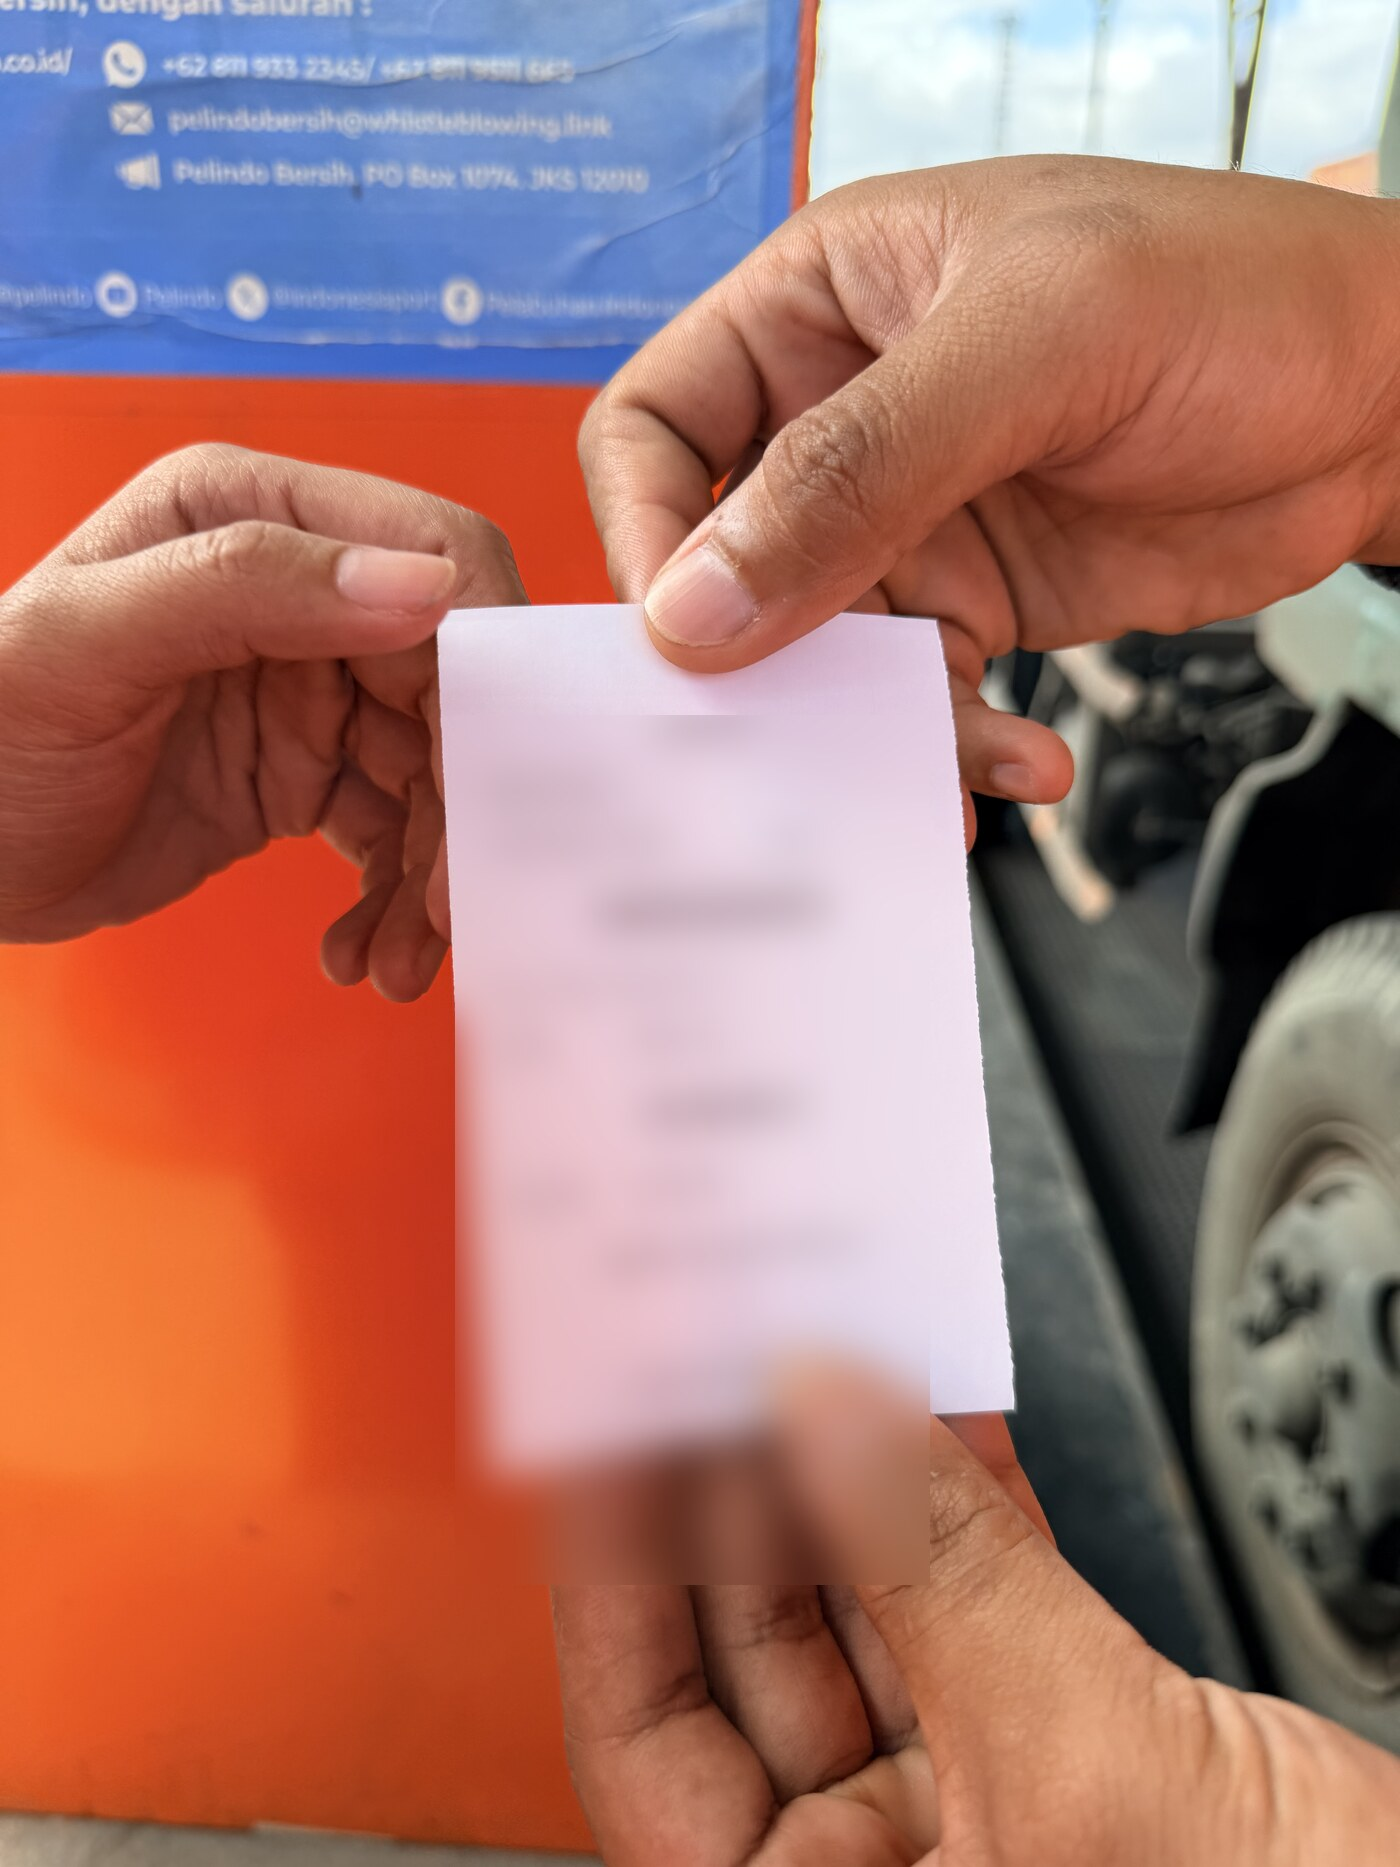
\includegraphics[height=0.18\textheight,width=\linewidth,keepaspectratio]{images/evidence-eksisting-dokumen-printout.jpg}
    \caption{Dokumen cetak}
    \label{fig:evidence_eksisting_dokumen_printout}
  \end{subfigure}
  \hfill
  \begin{subfigure}[t]{0.32\textwidth}
    \centering
    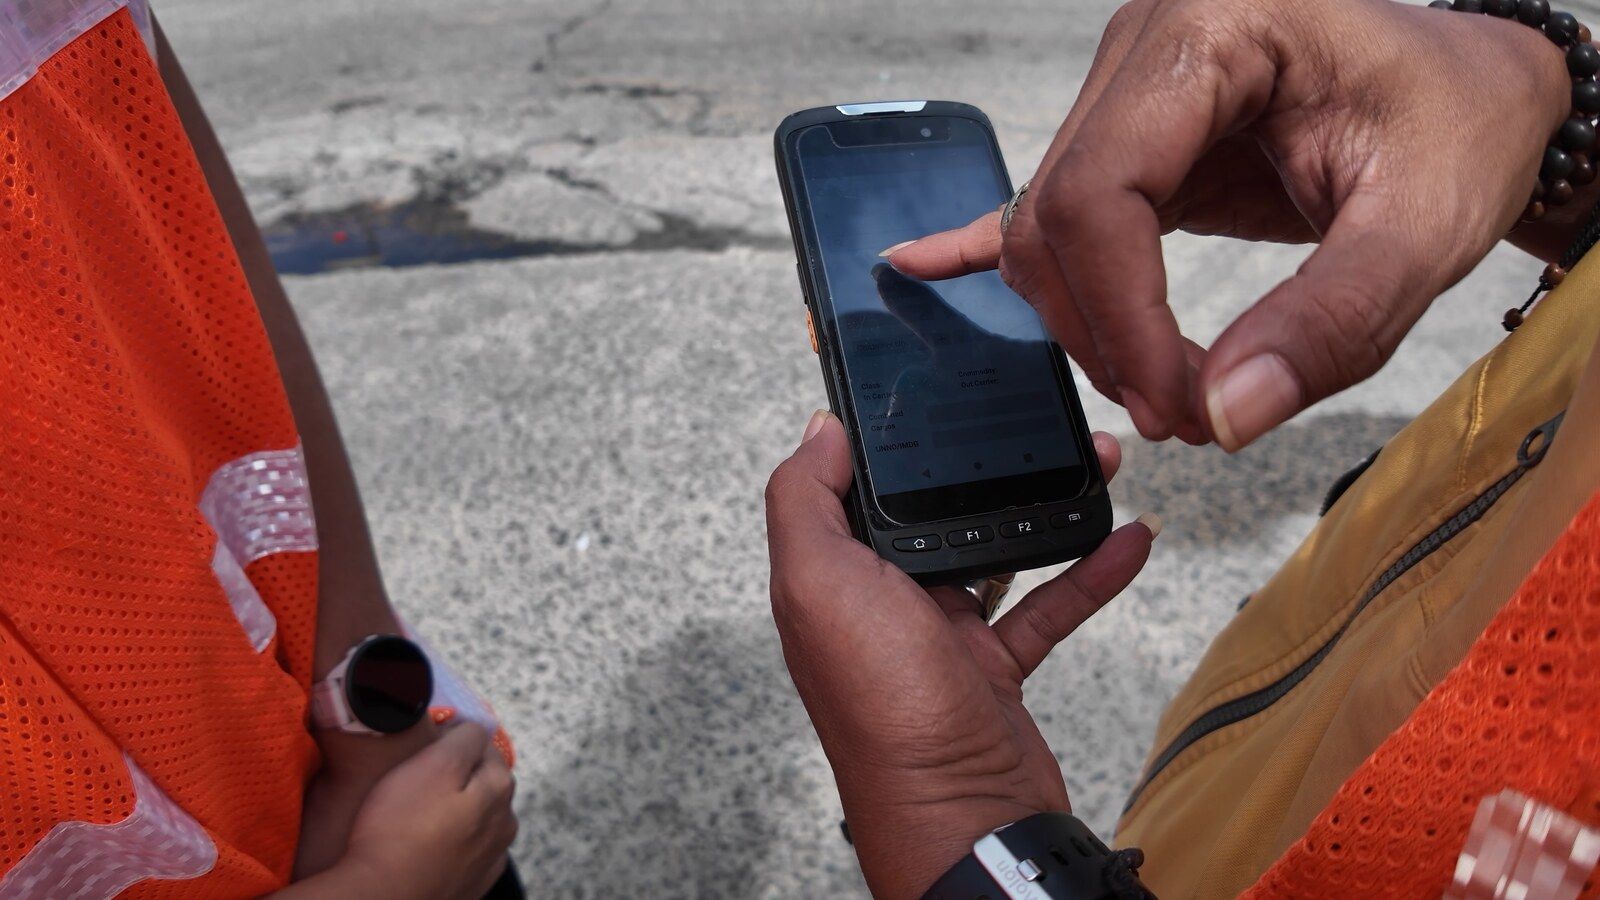
\includegraphics[height=0.18\textheight,width=\linewidth,keepaspectratio]{images/evidence-eksisting-pencatatan-mobile.jpg}
    \caption{Pencatatan mobile}
    \label{fig:evidence_eksisting_pencatatan_mobile}
  \end{subfigure}
  \hfill
  \begin{subfigure}[t]{0.32\textwidth}
    \centering
    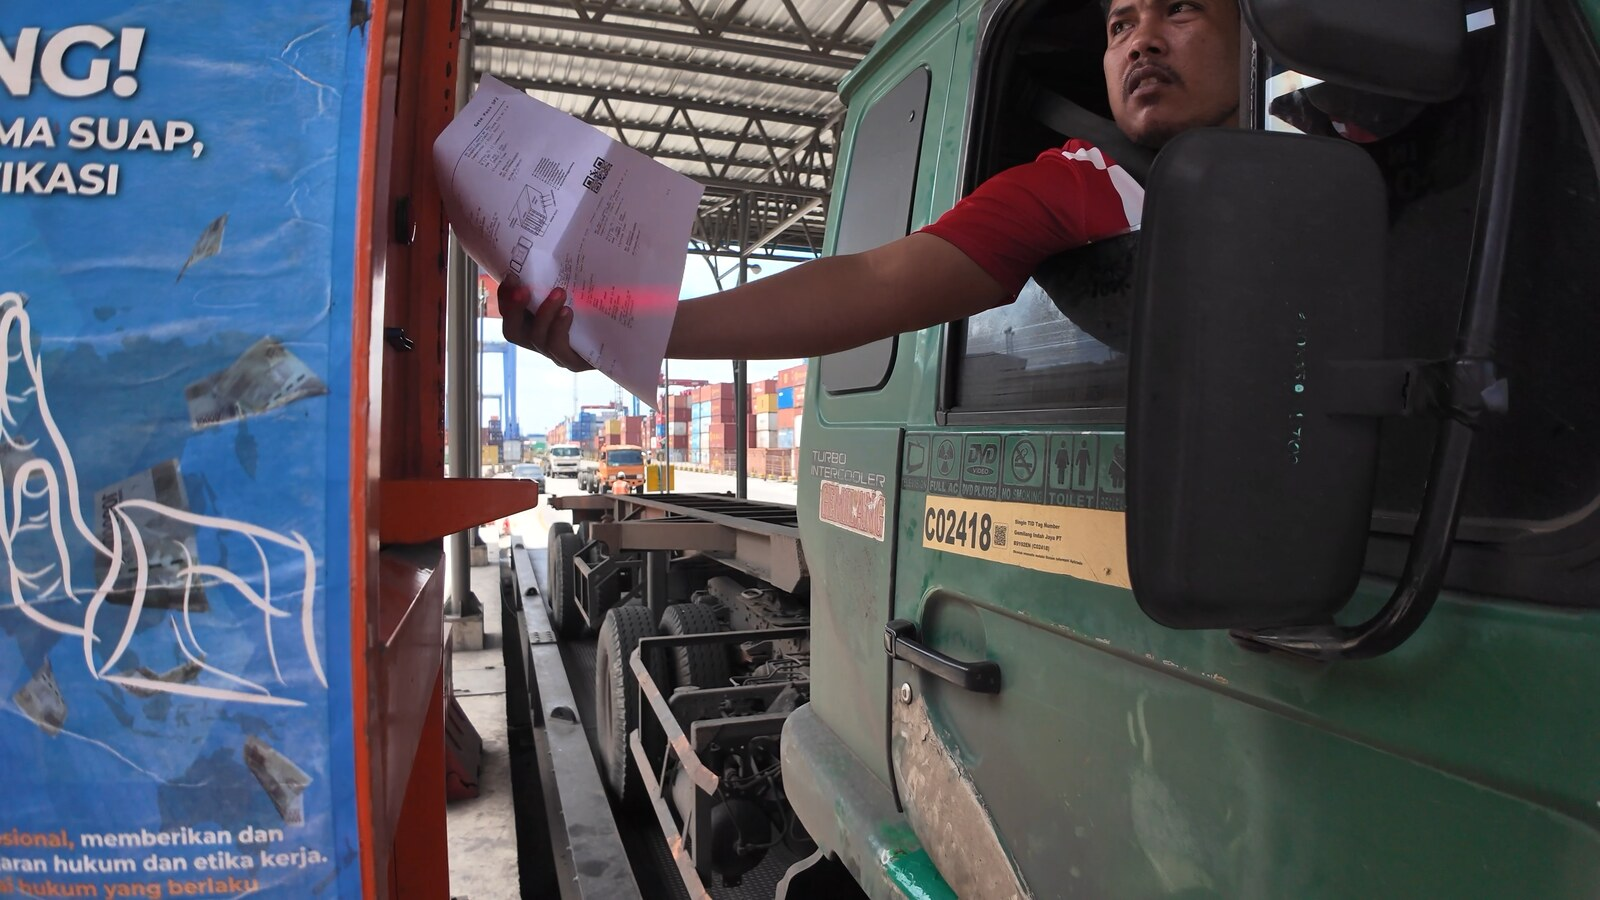
\includegraphics[height=0.18\textheight,width=\linewidth,keepaspectratio]{images/evidence-eksisting-form-manual.jpg}
    \caption{Interaksi dokumen}
    \label{fig:evidence_eksisting_form_manual}
  \end{subfigure}
  \caption{Bukti keterlibatan dokumen fisik dan pencatatan lapangan pada proses eksisting}
  \label{fig:evidence_eksisting_pencatatan_lapangan}
\end{figure}

Gambar~\ref{fig:evidence_eksisting_pencatatan_lapangan} menunjukkan bahwa
proses eksisting tidak hanya bergantung pada pemeriksaan fisik, tetapi juga
melibatkan dokumen cetak dan pencatatan lapangan. Pada dokumentasi perangkat
mobile, isi layar tidak digunakan sebagai bukti jenis platform karena pantulan
cahaya dan keterbatasan akses membuat identitas aplikasi tidak dapat dipastikan.
Dengan demikian, klaim analisis dibatasi pada penggunaan pencatatan mobile,
bukan pada penggunaan platform pencatatan tertentu.

\begin{table}[ht]
\centering
\scriptsize
\caption{Ringkasan Bukti Observasi Kondisi Eksisting}
\label{tbl:bukti_observasi_eksisting}
\begin{tabularx}{\textwidth}{>{\raggedright\arraybackslash}p{0.22\textwidth} >{\raggedright\arraybackslash}X >{\raggedright\arraybackslash}X >{\raggedright\arraybackslash}X}
\toprule
\textbf{Bukti Observasi} & \textbf{Temuan yang Didukung} & \textbf{Batasan Publikasi} & \textbf{Implikasi Kebutuhan Sistem} \\
\midrule
Pemeriksaan fisik kontainer & Inspeksi dilakukan langsung pada sisi kontainer oleh petugas lapangan & Nomor kontainer tidak selalu terlihat pada dokumentasi & Sistem perlu mengaitkan bukti visual dengan identitas kontainer dan status inspeksi \\
Dokumen cetak operasional & Proses masih melibatkan dokumen fisik sebagai referensi atau bukti operasional & Isi dokumen dan identitas operasional disamarkan karena memuat data terbatas & Sistem perlu menyediakan penyimpanan bukti dan struktur data yang mengurangi ketergantungan pada dokumen terpisah \\
Perangkat mobile di lapangan & Terdapat pencatatan atau pengisian data melalui perangkat mobile & Jenis aplikasi tidak diidentifikasi secara spesifik & Sistem perlu menyediakan formulir inspeksi terstruktur yang dapat digunakan di lapangan \\
Interaksi dokumen manual & Pertukaran dokumen masih terjadi pada titik layanan operasional & Detail isi formulir tidak ditampilkan karena keterbatasan akses & Sistem perlu menyediakan alur validasi, audit, dan riwayat kontainer yang terdokumentasi \\
\bottomrule
\end{tabularx}
\end{table}

\FloatBarrier

Model interaksi antaraktor dan titik masalah utama pada sistem manual diringkas
pada Gambar~\ref{fig:model_konseptual_saat_ini}.

\begin{figure}[ht]
  \centering
  \resizebox{0.98\textwidth}{!}{%
  \begin{tikzpicture}[
      font=\scriptsize,
      entity/.style={rectangle, rounded corners, draw=black, very thick, align=center, minimum width=2.70cm, minimum height=1.05cm},
      activity/.style={rectangle, draw=black, align=center, minimum width=2.70cm, minimum height=0.88cm},
      actor/.style={rectangle, draw=black, align=center, minimum width=2.40cm, minimum height=0.76cm},
      issue/.style={rectangle, rounded corners, draw=black, align=center, minimum width=2.75cm, minimum height=0.82cm},
      flow/.style={-{Latex[length=2.1mm,width=1.6mm]}, thick, rounded corners=2pt, line cap=round},
      weakflow/.style={-{Latex[length=2.0mm,width=1.5mm]}, dashed, thick, rounded corners=2pt, line cap=round}
    ]
    \node[entity] (kontainer) at (0,0) {\textbf{Kontainer}\\objek utama};

    \node[activity] (inspeksi) at (-3.75,0) {Pemeriksaan\\visual fisik};
    \node[actor] (petugas) at (-3.75,1.55) {Petugas\\Inspeksi};
    \node[activity] (checklist) at (-3.75,-1.55) {\textit{Checklist}\\manual};

    \node[activity] (catatan) at (3.75,0) {Dokumen kertas /\\catatan mobile};
    \node[activity] (riwayat) at (0,-1.75) {Riwayat kontainer\\belum terkonsolidasi};

    \node[actor, minimum width=3.20cm, minimum height=1.08cm] (penerima) at (8.20,0) {Distribusi manual\\Supervisor, Bea Cukai,\\dan email};
    \node[actor] (tos) at (8.20,-1.65) {TOS / PCS\\belum terintegrasi};

    \node[issue] (validasi) at (-7.35,-1.55) {Validasi dan standar\\data/proses\\belum tersedia};
    \node[issue] (audit) at (0,-3.30) {\textit{Audit trail} dan\\\textit{metadata} belum konsisten};
    \node[issue] (manual) at (8.20,-3.35) {Pertukaran data\\manual antarsistem};

    \draw[flow] (petugas) -- (inspeksi);
    \draw[flow] (checklist) -- (inspeksi);
    \draw[flow] (inspeksi) -- (kontainer);
    \draw[flow] (kontainer) -- (catatan);
    \draw[weakflow] (kontainer.south) -- (riwayat.north);
    \draw[weakflow] ([xshift=-0.50cm]catatan.south) |- (riwayat.east);

    \draw[flow] (catatan.east) -- (penerima.west);
    \draw[weakflow] ([xshift=0.50cm]catatan.south) |- (tos.west);

    \draw[weakflow] (validasi.east) -- (checklist.west);
    \draw[weakflow] (audit.north) -- (riwayat.south);
    \draw[weakflow] (manual.north) -- (tos.south);
  \end{tikzpicture}}
  \caption{Model konseptual sistem inspeksi kontainer saat ini serta titik permasalahan utama}
  \label{fig:model_konseptual_saat_ini}
\end{figure}

\subsection{Identifikasi Masalah Arsitektural}

Analisis terhadap model konseptual sistem saat ini menghasilkan identifikasi tiga kategori masalah arsitektural. Kategorisasi ini disusun berdasarkan pengelompokan tematik terhadap keterbatasan yang teridentifikasi pada dimensi \textit{people}, \textit{process}, \textit{technology}, dan \textit{data}. Setiap kategori masalah mencerminkan celah arsitektural yang menghambat pencapaian standardisasi, integrasi, dan keandalan operasional.

\textbf{Masalah standardisasi proses.}
Ketiadaan mekanisme standardisasi formal menyebabkan beberapa masalah berikut:

\begin{enumerate}
  \item Konsistensi hasil inspeksi rendah karena sistem belum memiliki definisi
  formal mengenai kategori kerusakan, tingkat keparahan, atau kriteria keputusan
  inspeksi.
  \item Subjektivitas hasil inspeksi tinggi karena penilaian masih bergantung
  pada interpretasi personal petugas tanpa panduan objektif yang terintegrasi.
  \item Belum terdapat komponen sistem yang memverifikasi kelengkapan atau
  kebenaran data inspeksi sebelum digunakan sebagai dasar pengambilan keputusan.
\end{enumerate}

\textbf{Masalah integrasi dan interoperabilitas.}
Isolasi sistem inspeksi dari ekosistem informasi pelabuhan menyebabkan beberapa
masalah berikut:

\begin{enumerate}
  \item Data inspeksi belum dapat diakses secara waktu nyata oleh sistem TOS,
  PCS, maupun pemangku kepentingan lain.
  \item Data yang sama sering kali harus dimasukkan ulang ke beberapa sistem,
  sehingga risiko kesalahan dan inkonsistensi meningkat.
  \item Belum terdapat antarmuka atau protokol komunikasi yang memungkinkan
  pertukaran data inspeksi secara otomatis dan mengikuti standar.
\end{enumerate}

\textbf{Masalah ketahanan dan keandalan operasional.}
Ketergantungan penuh pada proses manual membuat keandalan operasional rentan
terhadap beberapa kondisi berikut:

\begin{enumerate}
  \item Ketersediaan proses sangat bergantung pada petugas dan belum memiliki
  mekanisme cadangan yang memadai.
  \item Gangguan administrasi atau keterbatasan sumber daya dapat menghambat
  kontinuitas inspeksi.
  \item Proses belum memiliki kapabilitas untuk menyesuaikan kapasitas
  pemrosesan terhadap fluktuasi beban kerja.
\end{enumerate}

Berdasarkan model konseptual dan tiga kategori masalah arsitektural tersebut,
dapat disimpulkan bahwa sistem inspeksi kontainer saat ini belum menyediakan
standardisasi proses, integrasi lintas sistem, dan keandalan
operasional yang diperlukan untuk mendukung efisiensi layanan kepelabuhanan.
Temuan ini menjadi landasan untuk merumuskan kebutuhan sistem pada subbab
berikutnya.

\section{Analisis Kebutuhan Sistem}

Temuan pada sistem saat ini diterjemahkan menjadi kebutuhan sistem yang merespons celah arsitektural secara langsung. Analisis kebutuhan dibagi menjadi dua kategori: kebutuhan fungsional yang mendefinisikan kapabilitas sistem, dan kebutuhan nonfungsional yang menentukan atribut kualitas agar sistem dapat beroperasi secara andal dalam konteks pelabuhan Indonesia.

\subsection{Kebutuhan Fungsional}

Kebutuhan fungsional diturunkan dari tiga masalah arsitektural utama yang telah
diidentifikasi: standardisasi proses, integrasi informasi, dan keandalan
operasional. Tabel~\ref{tbl:kebutuhan_fungsional} merangkum kebutuhan
fungsional yang dikategorikan berdasarkan domain fungsional utama dalam
skenario operasional pelabuhan.

\begin{table}[ht]
\centering
\scriptsize
\caption{Kebutuhan Fungsional Sistem Inspeksi Kontainer}
\label{tbl:kebutuhan_fungsional}
\begin{tabular}{p{0.09\textwidth} p{0.18\textwidth} p{0.50\textwidth} p{0.09\textwidth}}
\toprule
\textbf{Kode} & \textbf{Domain} & \textbf{Kebutuhan} & \textbf{Prioritas} \\
\midrule
\textbf{FR-01} & \makecell[l]{Pencatatan\\Inspeksi} & Sistem mencatat hasil inspeksi berdasarkan standar formal yang terdokumentasi & Tinggi \\
\textbf{FR-02} & \makecell[l]{Pencatatan\\Inspeksi} & Sistem melacak riwayat inspeksi tiap kontainer beserta waktu dan penanggung jawab & Tinggi \\
\textbf{FR-03} & \makecell[l]{Pencatatan\\Inspeksi} & Sistem menyediakan visualisasi hasil inspeksi untuk dokumentasi dan audit & Tinggi \\
\textbf{FR-04} & \makecell[l]{Standardisasi\\Proses} & Sistem mendukung representasi hasil penilaian kerusakan berdasarkan kategori dan tingkat keparahan yang konsisten & Tinggi \\
\textbf{FR-05} & \makecell[l]{Standardisasi\\Proses} & Sistem mendukung validasi kelengkapan data inspeksi melalui struktur data dan alur proses yang terdefinisi & Tinggi \\
\textbf{FR-06} & \makecell[l]{Standardisasi\\Proses} & Sistem menjaga konsistensi interpretasi hasil antarpetugas & Tinggi \\
\textbf{FR-07} & \makecell[l]{Integrasi\\Data} & Sistem menyediakan pola antarmuka pertukaran data yang dapat dikembangkan untuk integrasi dengan Terminal Operating System & Tinggi \\
\textbf{FR-08} & \makecell[l]{Integrasi\\Data} & Sistem menyediakan akses terstruktur terhadap hasil inspeksi bagi pemangku kepentingan yang berwenang & Tinggi \\
\textbf{FR-09} & \makecell[l]{Integrasi\\Data} & Sistem menyajikan akses terstruktur untuk pelaporan dan analitik & Sedang \\
\textbf{FR-10} & \makecell[l]{Tata Kelola\\dan Audit} & Sistem membangun \textit{audit trail} lengkap untuk seluruh aktivitas inspeksi & Tinggi \\
\textbf{FR-11} & \makecell[l]{Tata Kelola\\dan Audit} & Sistem mengelola pengguna dengan kontrol akses berbasis peran & Tinggi \\
\bottomrule
\end{tabular}
\end{table}

\FloatBarrier

Domain fungsional tersebut disusun dengan mengacu pada panduan kondisi kontainer
seperti IICL dan UCIRC, checklist keamanan kontainer CTPAT, serta kerangka
keamanan perdagangan internasional (\textit{WCO SAFE Framework}). Acuan tersebut
kemudian disesuaikan dengan konteks operasional pelabuhan Indonesia sesuai
Peraturan Menteri Perhubungan No.~8/2022.

\subsection{Kebutuhan Nonfungsional}

Kebutuhan nonfungsional mendefinisikan atribut kualitas yang menjadi sasaran rancangan agar sistem dapat dikembangkan menuju operasi yang andal dan terukur dalam konteks pelabuhan Indonesia. Tabel~\ref{tbl:kebutuhan_nonfungsional} merangkum kebutuhan nonfungsional berdasarkan kelompok kapabilitas inti ISO/IEC 25010 dan karakteristik operasional pelabuhan.

\begin{table}[ht]
\centering
\scriptsize
\caption{Kebutuhan Nonfungsional Sistem Inspeksi Kontainer}
\label{tbl:kebutuhan_nonfungsional}
\begin{tabular}{p{0.10\textwidth} p{0.18\textwidth} p{0.62\textwidth}}
\toprule
\textbf{Kode} & \textbf{Atribut Kualitas} & \textbf{Deskripsi Kebutuhan} \\
\midrule
\textbf{NFR-01} & \makecell[l]{\textit{Performance}\\\textit{Efficiency}}
& Sistem merespons permintaan pengguna dalam waktu yang wajar. Efisiensi pemrosesan data dijaga meskipun volume data inspeksi meningkat seiring ekspansi operasional. \\
\textbf{NFR-02} & \textit{Interoperability}
& Arsitektur sistem menyediakan batas antarmuka dan pola pertukaran data yang memungkinkan integrasi bertahap dengan berbagai sistem pelabuhan (TOS, PCS, Inaportnet) tanpa mengubah logika inti sistem. \textit{Interface} integrasi dirancang mengikuti format data yang konsisten dan mudah dipetakan ke standar industri logistik. \\
\textbf{NFR-03} & \textit{Reliability}
& Sistem beroperasi secara konsisten dalam kondisi infrastruktur heterogen. Keandalan operasional dijaga meskipun terjadi gangguan koneksi atau keterbatasan infrastruktur di lokasi pelabuhan tertentu. Ketersediaan sistem dijaga melalui mekanisme toleransi kesalahan dan pemulihan yang efektif. \\
\textbf{NFR-04} & \textit{Security}
& Sistem menyediakan mekanisme untuk melindungi integritas dan kerahasiaan data inspeksi. Akses terhadap data dan fungsi sistem dikontrol berdasarkan prinsip \textit{least privilege}. \\
\textbf{NFR-05} & \textit{Maintainability}
& Arsitektur sistem mendukung modifikasi dan evolusi dengan upaya minimal. Pemisahan tanggung jawab yang jelas antarkomponen dijaga untuk memfasilitasi pemeliharaan jangka panjang. Sistem memiliki tingkat \textit{modifiability} yang memadai untuk adaptasi terhadap perubahan regulasi atau kebutuhan operasional tanpa perancangan ulang menyeluruh. \\
\bottomrule
\end{tabular}
\end{table}

\FloatBarrier

Atribut kualitas tersebut dipilih karena merepresentasikan faktor kritis keberhasilan sistem otomasi inspeksi dan selaras dengan prinsip arsitektur sistem terdistribusi yang telah dipaparkan dalam Bab II.

\section{Alternatif Solusi Konseptual}

Berdasarkan kebutuhan sistem yang telah ditetapkan, lima alternatif solusi
konseptual dirumuskan untuk membandingkan pendekatan desain yang meningkatkan
standardisasi proses, integrasi informasi, dan keandalan
operasional sistem inspeksi kontainer. Setiap alternatif dianalisis berdasarkan
prinsip desain, kelebihan, dan keterbatasannya dalam konteks operasional
pelabuhan Indonesia.

Rumusan alternatif juga memanfaatkan insight studi banding terhadap model
rujukan pada Bab II. Sistem \textit{GateCCR} dari TMEIC memberi rujukan bahwa
identifikasi visual kontainer di area gerbang dapat diperlakukan sebagai titik
akuisisi data yang terhubung dengan operasi terminal \autocite{tmeic2023}.
Solusi \textit{Visy ADDS} menunjukkan bahwa inspeksi kerusakan kontainer perlu
ditempatkan sebagai alur pemindaian visual yang menghasilkan bukti dan harus
dikaitkan ke identitas kontainer
\autocite{visy2023}. Kerangka WCO SAFE menekankan alur berbasis risiko dan
pertukaran informasi; ISO/IEC 25010 memberi dasar atribut kualitas; sedangkan
literatur arsitektur layanan dan \textit{edge-cloud} memberi rujukan pembagian
fungsi lokal-terpusat.

Dari studi banding tersebut, insight yang digunakan pada analisis adalah bahwa
nomor kontainer perlu menjadi jangkar integrasi, bukti visual perlu dipisahkan
dari data inti tetapi tetap tertaut pada kontainer, pemrosesan dekat sumber data
perlu dipisahkan dari penyimpanan terpusat, dan integrasi eksternal perlu
ditempatkan sebagai lapisan adaptor agar sistem inti tidak bergantung langsung
pada TOS, PCS, atau Inaportnet. Insight tersebut diterjemahkan menjadi lima
pilihan arsitektur agar pembahasan tidak berhenti pada daftar teknologi, tetapi
menunjukkan model rujukan yang dapat dipakai untuk memilih pola rancangan.

Perbedaan konseptual kelima alternatif diringkas pada
Tabel~\ref{tbl:perbedaan-konseptual-alternatif}. Ringkasan ini digunakan agar
pembaca dapat melihat bahwa alternatif yang dibandingkan bukan sekadar variasi
nama, tetapi memiliki pusat perhatian, bentuk komponen, dan implikasi
arsitektural yang berbeda.

\begin{table}[ht]
\centering
\scriptsize
\caption{Perbedaan Konseptual Alternatif Solusi}
\label{tbl:perbedaan-konseptual-alternatif}
\setlength{\tabcolsep}{3pt}
\renewcommand{\arraystretch}{1.08}
\begin{tabularx}{\textwidth}{>{\raggedright\arraybackslash}p{0.18\textwidth} >{\raggedright\arraybackslash}X >{\raggedright\arraybackslash}X >{\raggedright\arraybackslash}X}
\toprule
\textbf{Alternatif} & \textbf{Pusat Desain} & \textbf{Bentuk Komponen Utama} & \textbf{Implikasi Arsitektural} \\
\midrule
Standardisasi proses dan data & Keseragaman tahapan inspeksi dan format data & Modul mengikuti urutan pencatatan, validasi, dan pelaporan & Kuat untuk konsistensi prosedur, tetapi integrasi eksternal masih perlu dirancang terpisah \\
Integrasi terorkestrasi & Pertukaran informasi antarsistem & Layanan tematik yang dikoordinasikan oleh lapisan orkestrasi & Kuat untuk interoperabilitas, tetapi membutuhkan tata kelola kontrak layanan yang ketat \\
Modular berbasis domain & Pemisahan tanggung jawab berdasarkan domain inspeksi & Modul akuisisi, analisis, otorisasi, pelaporan, dan integrasi dengan antarmuka jelas & Seimbang untuk modularitas, evolusi sistem, dan integrasi bertahap \\
Alur kerja berbasis peristiwa & Perubahan status sebagai pemicu proses & Produsen dan konsumen \textit{event} dengan \textit{payload} yang mengikuti standar & Responsif dan mudah diaudit, tetapi kompleksitas skema \textit{event} harus dijaga \\
Tata kelola data terpadu & Kepemilikan, kualitas, dan \textit{lineage} data & Registri \textit{metadata}, layanan kualitas data, dan mekanisme persetujuan & Kuat untuk audit dan kepatuhan, tetapi membutuhkan kesiapan organisasi yang tinggi \\
\bottomrule
\end{tabularx}
\end{table}

\FloatBarrier

Selain melalui tabel, perbedaan kelima alternatif juga perlu dibaca sebagai
perbedaan pusat keputusan arsitektural. Gambar~\ref{fig:peta-alternatif-solusi}
memperlihatkan bahwa setiap alternatif berangkat dari lensa desain yang berbeda,
yaitu proses, integrasi, domain, peristiwa, atau tata kelola data. Pemetaan ini
digunakan sebagai dasar untuk memilih alternatif yang paling sesuai dengan
kontribusi tugas akhir, yaitu perancangan arsitektur sistem inspeksi kontainer
yang terintegrasi namun tetap modular.

\begin{figure}[htbp]
  \centering
  \resizebox{0.98\textwidth}{!}{%
  \begin{tikzpicture}[
      font=\scriptsize,
      altbox/.style={rectangle, rounded corners, draw=black, align=center, minimum width=3.05cm, minimum height=1.05cm},
      chosen/.style={rectangle, rounded corners, draw=black, very thick, align=center, minimum width=3.05cm, minimum height=1.05cm},
      note/.style={rectangle, draw=black, align=center, minimum width=3.05cm, minimum height=0.68cm},
      line/.style={-{Latex[length=1.8mm]}, thick}
    ]
    \node[altbox] (a1) at (0,0) {\textbf{Alternatif 1}\\Standardisasi\\Proses dan Data};
    \node[altbox] (a2) at (3.55,0) {\textbf{Alternatif 2}\\Integrasi\\Terorkestrasi};
    \node[chosen] (a3) at (7.10,0) {\textbf{Alternatif 3}\\Modular\\Berbasis Domain};
    \node[altbox] (a4) at (10.65,0) {\textbf{Alternatif 4}\\Alur Kerja\\Berbasis Peristiwa};
    \node[altbox] (a5) at (14.20,0) {\textbf{Alternatif 5}\\Tata Kelola\\Data Terpadu};

    \node[note, below=0.55cm of a1] (n1) {Lensa utama:\\tahapan inspeksi};
    \node[note, below=0.55cm of a2] (n2) {Lensa utama:\\pertukaran data};
    \node[note, below=0.55cm of a3] (n3) {Lensa utama:\\batas tanggung jawab};
    \node[note, below=0.55cm of a4] (n4) {Lensa utama:\\perubahan status};
    \node[note, below=0.55cm of a5] (n5) {Lensa utama:\\kepemilikan data};

    \node[note, below=0.42cm of n1] (m1) {Komponen mengikuti\\urutan proses};
    \node[note, below=0.42cm of n2] (m2) {Komponen dipusatkan\\pada orkestrasi};
    \node[note, below=0.42cm of n3] (m3) {Komponen dipisah\\berdasarkan domain};
    \node[note, below=0.42cm of n4] (m4) {Komponen bereaksi\\terhadap \textit{event}};
    \node[note, below=0.42cm of n5] (m5) {Komponen menjaga\\kualitas dan \textit{lineage}};

    \draw[line] (a1) -- (n1);
    \draw[line] (a2) -- (n2);
    \draw[line] (a3) -- (n3);
    \draw[line] (a4) -- (n4);
    \draw[line] (a5) -- (n5);
    \draw[line] (n1) -- (m1);
    \draw[line] (n2) -- (m2);
    \draw[line] (n3) -- (m3);
    \draw[line] (n4) -- (m4);
    \draw[line] (n5) -- (m5);
  \end{tikzpicture}}
  \caption{Peta Perbedaan Konseptual Alternatif Solusi}
  \label{fig:peta-alternatif-solusi}
\end{figure}

\FloatBarrier

\subsection{Ringkasan Kelebihan dan Keterbatasan Alternatif}

Uraian rinci setiap alternatif diringkas pada Tabel
\ref{tbl:ringkasan-alternatif-solusi} agar perbandingan lebih langsung
terhubung dengan kriteria evaluasi pada bagian berikutnya. Ringkasan ini
menjaga tiga aspek yang diperlukan untuk pemilihan solusi: pusat desain,
kelebihan utama, dan keterbatasan utama.

\begin{table}[htbp]
\centering
\scriptsize
\caption{Ringkasan Kelebihan dan Keterbatasan Alternatif Solusi}
\label{tbl:ringkasan-alternatif-solusi}
\setlength{\tabcolsep}{3pt}
\renewcommand{\arraystretch}{1.10}
\begin{tabularx}{\textwidth}{>{\raggedright\arraybackslash}p{0.20\textwidth} >{\raggedright\arraybackslash}X >{\raggedright\arraybackslash}X}
\toprule
\textbf{Alternatif} & \textbf{Kelebihan Utama} & \textbf{Keterbatasan Utama} \\
\midrule
Standardisasi proses dan data & Menyeragamkan tahapan inspeksi, format data, dan dasar audit sejak pencatatan awal. & Belum cukup kuat untuk interoperabilitas eksternal apabila tidak disertai rancangan orkestrasi informasi. \\
Integrasi terorkestrasi & Menempatkan kontrak pertukaran data dan koordinasi antarlayanan sebagai pusat rancangan. & Memerlukan tata kelola kontrak layanan yang ketat dan kesiapan perubahan lintas unit. \\
Modular berbasis domain & Memisahkan akuisisi, analisis, otorisasi, pelaporan, dan integrasi sehingga perubahan dapat dilakukan bertahap. & Membutuhkan disiplin dokumentasi antarmodul agar modularitas tidak berubah menjadi silo fungsional. \\
Alur kerja berbasis peristiwa & Mencatat perubahan status sebagai \textit{event} sehingga proses lebih reaktif dan mudah diaudit. & Kompleksitas skema \textit{event} dan pemantauan pesan perlu dikendalikan agar status tidak terpecah. \\
Tata kelola data terpadu & Memperkuat kepemilikan data, kualitas informasi, \textit{lineage}, dan mekanisme persetujuan. & Membutuhkan kesiapan organisasi tinggi dan dapat menjadi birokratis bila tidak selaras dengan operasi harian. \\
\bottomrule
\end{tabularx}
\end{table}

\FloatBarrier

\section{Analisis Pemilihan Solusi}

Pemilihan solusi dilakukan melalui evaluasi terstruktur terhadap lima alternatif konseptual berdasarkan kriteria yang diturunkan dari kebutuhan sistem dan prinsip arsitektur yang telah dipaparkan dalam Bab II.

\subsection{Kriteria Evaluasi}

Kriteria evaluasi disusun berdasarkan keselarasan dengan kebutuhan fungsional, kebutuhan nonfungsional (ISO/IEC 25010), dan prinsip arsitektur sistem terdistribusi. Tabel~\ref{tbl:kriteria_evaluasi} merangkum kriteria evaluasi beserta definisinya.

\begin{table}[ht]
\centering
\footnotesize
\caption{Kriteria Evaluasi Alternatif Solusi}
\label{tbl:kriteria_evaluasi}
\setlength{\tabcolsep}{4pt}
\renewcommand{\arraystretch}{1.12}
\begin{tabularx}{\textwidth}{>{\raggedright\arraybackslash}p{0.22\textwidth} >{\raggedright\arraybackslash}X >{\raggedright\arraybackslash}p{0.22\textwidth}}
\toprule
\textbf{Kriteria} & \textbf{Indikator Penilaian} & \textbf{Dasar Skor Tinggi} \\
\midrule
Keselarasan Proses & Alternatif menyediakan tahapan inspeksi, status proses, dan aturan perpindahan aktivitas yang dapat dipakai lintas petugas. & Proses tercatat eksplisit dan mengurangi variasi interpretasi. \\
Interoperabilitas & Alternatif memisahkan kontrak pertukaran data dari logika inspeksi inti sehingga TOS, PCS, Inaportnet, atau sistem eksternal dapat dipetakan bertahap. & Integrasi eksternal dapat ditambahkan tanpa merombak domain inspeksi utama. \\
Modularitas Komponen & Alternatif membagi tanggung jawab komponen berdasarkan batas domain, jenis data, dan kebutuhan pemrosesan. & Perubahan pada satu komponen tidak memaksa perubahan menyeluruh pada komponen lain. \\
Tata Kelola Data & Alternatif menjaga keterkaitan identitas kontainer, hasil inspeksi, bukti visual, dan jejak aktivitas. & Riwayat kontainer dapat ditelusuri dari data dan artefak bukti. \\
Keberlanjutan Operasional & Alternatif menyediakan pemisahan beban kerja dan jalur komunikasi agar gangguan pada satu bagian tidak langsung menghentikan seluruh fungsi. & Operasi dapat dilanjutkan atau dipulihkan berdasarkan batas komponen yang jelas. \\
\bottomrule
\end{tabularx}
\end{table}

\FloatBarrier

Kriteria-kriteria ini mewakili faktor kritis keberhasilan rancangan sistem otomasi inspeksi kontainer dan selaras dengan atribut kualitas yang direkomendasikan oleh ISO/IEC 25010 serta prinsip arsitektur sistem terdistribusi.

\subsection{Matriks Perbandingan Alternatif}

Evaluasi dilakukan dengan penilaian kualitatif yang diterjemahkan menjadi skala numerik 1 hingga 4, merepresentasikan tingkat kesesuaian alternatif dengan setiap kriteria: 1 (sangat rendah), 2 (rendah), 3 (sedang), 4 (tinggi). Skor tersebut digunakan sebagai alat bantu pengambilan keputusan desain, bukan sebagai hasil pengukuran kuantitatif terhadap performa sistem. Oleh karena itu, nilai pada matriks dibaca bersama uraian kelebihan, keterbatasan, dan kesesuaian setiap alternatif terhadap ruang lingkup tugas akhir. Tabel~\ref{tbl:evaluasi_alternatif} merangkum hasil evaluasi terhadap kelima alternatif solusi.

\begin{table}[ht]
\centering
\small
\caption{Matriks Evaluasi Alternatif Solusi}
\label{tbl:evaluasi_alternatif}
\begin{tabular}{p{0.30\textwidth} p{0.08\textwidth} p{0.08\textwidth} p{0.08\textwidth} p{0.08\textwidth} p{0.08\textwidth} p{0.08\textwidth}}
\toprule
\textbf{Alternatif} & \textbf{Proc.} & \textbf{Int.} & \textbf{Mod.} & \textbf{Gov.} & \textbf{Sust.} & \textbf{Total} \\
\midrule
1. Standardisasi Proses dan Data & 4 & 2 & 2 & 3 & 3 & 14 \\
2. Integrasi Terorkestrasi & 3 & 4 & 3 & 3 & 3 & 16 \\
3. Modular Berbasis Domain & 3 & 3 & 4 & 3 & 4 & 17 \\
4. Alur Kerja Berbasis Peristiwa & 3 & 3 & 3 & 2 & 3 & 14 \\
5. Tata Kelola Data Terpadu & 3 & 3 & 2 & 4 & 3 & 15 \\
\bottomrule
\end{tabular}
\end{table}

\FloatBarrier

\textbf{Keterangan:} Proc.=Keselarasan proses, Int.=Interoperabilitas, Mod.=Modularitas komponen, Gov.=Tata kelola data, Sust.=Keberlanjutan operasional.

Hasil evaluasi menunjukkan bahwa \textbf{Alternatif 3: Arsitektur Modular Berbasis Domain} memperoleh skor total tertinggi (17) karena memberikan keseimbangan paling sesuai antara keselarasan proses, modularitas komponen, dan keberlanjutan operasional pada ruang lingkup perancangan arsitektur. Selisih terhadap alternatif integrasi terorkestrasi (skor 16) tidak dibaca sebagai perbedaan mutlak, melainkan sebagai indikasi bahwa kedua pendekatan memiliki penekanan berbeda. Alternatif integrasi terorkestrasi unggul pada interoperabilitas, namun membutuhkan tata kelola kontrak layanan lintas sistem yang lebih kompleks daripada ruang lingkup realisasi tugas akhir ini. Alternatif modular berbasis domain dipilih karena tetap memberi ruang integrasi bertahap sekaligus menjaga batas tanggung jawab komponen agar dapat direalisasikan dan dievaluasi melalui artefak sistem yang tersedia. Alternatif tata kelola data terpadu (skor 15) memiliki keunggulan pada aspek \textit{governance} tetapi kurang fleksibel dalam modularitas komponen. Dua alternatif lainnya cenderung fokus pada satu aspek tertentu sehingga kontribusinya terhadap kriteria lain lebih terbatas. Hasil ini mengindikasikan bahwa solusi terpilih menggabungkan struktur proses yang konsisten dengan komposisi komponen yang modular agar integrasi dan tata kelola data dapat berkembang secara berkelanjutan.

\subsection{Justifikasi Pemilihan Solusi}

Berdasarkan matriks evaluasi dan analisis terhadap karakteristik setiap alternatif, \textbf{Alternatif 3: Arsitektur Modular Berbasis Domain} dipilih sebagai solusi yang paling sesuai untuk mengatasi masalah sistem inspeksi kontainer di Indonesia. Justifikasi pemilihan disusun berdasarkan empat perspektif: kebutuhan operasional, atribut kualitas ISO/IEC 25010, prinsip arsitektur, dan kepatuhan terhadap standar dan regulasi.

\textbf{Justifikasi berdasarkan kebutuhan operasional.}
Kebutuhan operasional pelabuhan Indonesia menuntut keselarasan proses antar
pelabuhan tanpa menghilangkan ruang adaptasi lokal. Arsitektur modular
berbasis domain menjawab tuntutan tersebut dengan membagi alur inspeksi ke
dalam domain yang jelas, sehingga setiap pelabuhan menjalankan urutan proses
yang sama namun tetap memiliki keleluasaan mengelola detail operasional.
Pendekatan ini juga membuat tanggung jawab setiap domain, seperti pencatatan,
analisis, otorisasi, dan pelaporan, menjadi lebih eksplisit sehingga koordinasi
antaraktor lebih mudah dilakukan. Selain itu, perubahan kebijakan atau beban
kerja dapat diserap oleh domain yang terdampak tanpa mengganggu keseluruhan
sistem.

\textbf{Justifikasi berdasarkan atribut kualitas ISO/IEC 25010.}
Modularitas memberikan kontribusi langsung terhadap atribut kualitas yang
diprioritaskan dalam kebutuhan nonfungsional \autocite{bass2022}. Dari sisi
\textit{maintainability}, modul yang terisolasi mempermudah perbaikan dan
evolusi fungsional tanpa efek samping pada domain lain. Dari sisi
\textit{reliability}, keberlanjutan operasional lebih terjamin karena kegagalan
satu domain tidak meruntuhkan keseluruhan sistem. Dari sisi
\textit{interoperability}, kontrak antardomain dapat dirancang sebagai
antarmuka standar yang dapat diekspose ke sistem eksternal. Dari sisi
\textit{security}, struktur data yang mengikuti batas domain mendukung
penerapan kontrol akses berbasis domain dan meminimalkan risiko inkonsistensi.

\textbf{Justifikasi berdasarkan prinsip arsitektur.}
Prinsip \textit{modularity} dan \textit{loose coupling} yang menjadi dasar
arsitektur ini selaras dengan rekomendasi literatur arsitektur sistem
\autocite{newman2015}. Setiap domain dapat berevolusi dengan siklus
pengembangan sendiri, sementara hubungan antardomain dijaga melalui kontrak
komunikasi yang terdokumentasi. Pendekatan ini juga memperkuat tata kelola
karena organisasi perlu mendokumentasikan batasan, antarmuka, dan dependensi
sejak tahap konseptual. Di samping itu, penerapan \textit{domain boundary}
menyelaraskan aspek \textit{people} dan \textit{technology}, karena tim proses
dapat memfokuskan perbaikan pada domain masing-masing, sedangkan tim teknologi
memiliki peta komponen yang lebih jelas.

\textbf{Justifikasi berdasarkan standar dan regulasi.}
Penekanan pada modularitas dan peran domain juga memudahkan pemetaan
kebutuhan regulasi ke komponen sistem. Peraturan Menteri Perhubungan No.~8/2022
menunjukkan penggunaan Inaportnet sebagai layanan elektronik pelabuhan, dan
konteks tersebut dapat diterjemahkan ke dalam domain integrasi sebagai modul
khusus yang disiapkan untuk pertukaran data resmi \autocite{kemenhub2022}.
Prinsip tata kelola informasi dalam \textit{WCO SAFE Framework}
juga dapat diterjemahkan ke dalam domain tata kelola data yang
memegang kendali atas kualitas dan audit informasi \autocite{wco2025}. Dengan
struktur berbasis domain, setiap kewajiban regulatif memiliki pemilik yang
lebih jelas dalam arsitektur konseptual.

Berdasarkan justifikasi dari empat perspektif tersebut, arsitektur modular
berbasis domain memberikan fondasi yang kokoh untuk mengatasi tiga kategori
masalah arsitektural yang telah diidentifikasi: standardisasi proses, integrasi
lintas sistem, dan keandalan operasional.

\section{Kesimpulan Analisis}

Analisis yang telah dilakukan menghasilkan kesimpulan bahwa sistem inspeksi
kontainer saat ini menghadapi tiga masalah arsitektural utama: ketiadaan
standardisasi proses, fragmentasi informasi akibat isolasi sistem, dan
ketergantungan pada proses manual yang mengurangi keandalan operasional.

Eksplorasi terhadap lima alternatif solusi konseptual menunjukkan bahwa arsitektur modular berbasis domain memberikan keseimbangan paling sesuai antara keselarasan proses, modularitas komponen, dan tata kelola data pada ruang lingkup tugas akhir. Pemilihan solusi ini didasarkan pada evaluasi terstruktur terhadap kriteria yang diturunkan dari ISO/IEC 25010, prinsip arsitektur sistem terdistribusi, dan konteks operasional pelabuhan Indonesia.

Solusi yang dipilih menjadi fondasi untuk perancangan arsitektur konseptual
yang akan dipaparkan pada Bab IV, mencakup definisi domain komponen, alur
informasi antardomain, mekanisme integrasi standar, dan prinsip tata kelola
data yang mendukung ekosistem informasi pelabuhan. Bab berikutnya menerjemahkan
hasil analisis ini menjadi struktur arsitektur terperinci agar operasi
inspeksi kontainer dapat terotomasi secara terstruktur, mengikuti standar, dan
siap diintegrasikan.
